%-----------------------------------------------------------------------------%
\chapter{\babSatu}
%-----------------------------------------------------------------------------%


%-----------------------------------------------------------------------------%
\section{Latar Belakang}
%-----------------------------------------------------------------------------%
Badan Pusat Statistik (BPS) merupakan suatu lembaga pemerintah non-departemen yang bertanggung jawab dalam penyediaan statistik dasar di Indonesia \citep{bps_badan_2016}. Sebagai penyedia data, BPS melakukan pengumpulan data dengan menggunakan 2 (dua) metode, yaitu primer dan sekunder. Pengumpulan data primer dilakukan melalui wawancara langsung terhadap responden, baik responden individu, rumah tangga, maupun perusahaan. Di sisi lain, pengumpulan data sekunder dilakukan dengan melakukan kompilasi data yang telah dikumpulkan oleh pihak lain, tanpa adanya proses wawancara. 


Dalam pengumpulan data primer yang disebut dengan pencacahan, suatu wilayah administrasi dibagi menjadi beberapa Blok Sensus (BS). Blok Sensus merupakan satuan terkecil wilayah kerja dalam pencacahan.\citep{bps_sistem_2016}. Setiap petugas pencacahan memiliki beban tugas berupa 1 (satu) atau lebih BS. Pada setiap BS terdapat 1 (satu) atau lebih rumah tangga yang menjadi target pencacahan. \autoref{fig:capi-ilustration} memberikan ilustrasi pembagian BS dalam desa/kelurahan. 


\begin{figure}[!]
    \centering
    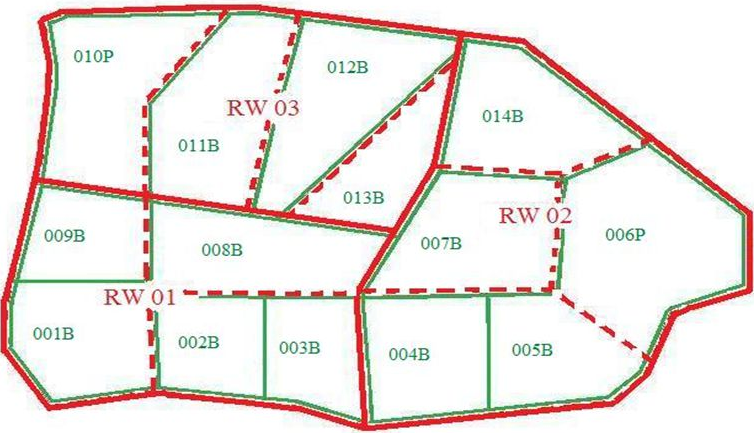
\includegraphics[width=10cm]{Resources/Images/peta_kelurahan_per_bs}
    \captionsetup{format=hang}
    \caption{Pembagian Blok Sensus dalam Desa/Kelurahan}
    \label{fig:capi-ilustration}
\end{figure}


Alokasi BS kepada setiap petugas pencacahan ditentukan oleh BPS sebagai \textit{subject matter} dengan memperhatikan kriteria berikut:
\begin{enumerate}
	\item Minimum total waktu dan biaya 
	\item Lokasi tugas relatif dekat dengan kantor BPS atau wilayah domisili petugas. 
\end{enumerate}
Pengalokasian BS dapat menjadi suatu hal yang problematik karena alokasi yang kurang cermat akan menyebabkan terjadinya ketimpangan pada total waktu penyelesaian pencacahan antar petugas. Kondisi ini dapat mengakibatkan terlambatnya kegiatan pencacahan secara keseluruhan.


Total waktu pencacahan merupakan akumulasi dari waktu tempuh antar wilayah kerja dan lama pencacahan dari seluruh wilayah kerja. Lama pencacahan pada suatu wilayah kerja  tersusun atas waktu tempuh antar rumah tangga dan lama wawancara pada seluruh rumah tangga di wilayah kerja tersebut. Berdasarkan \citep{sudman_time_1965}, komposisi waktu yang dihabiskan oleh seorang pencacah adalah 21 persen untuk berpindah antar wilayah kerja, 15 persen untuk berpindah antar rumah tangga, 15 persen untuk proses wawancara, dan sisanya untuk kegiatan lain seperti pengenalan wilayah dan perbaikan data.


Permasalahan alokasi wilayah kerja pencacahan memiliki kesamaan karakteristik dengan \textit{Vehicle Routing Problem} (VRP), khususnya \textit{Multi Depot Vehicle Routing Problem} (MDVRP). VRP merupakan suatu permasalahan penentuan rute terbaik yang harus ditempuh oleh beberapa kendaraan untuk mengirimkan barang kepada konsumen \citep{dantzig_truck_1959}. Sementara MDVRP adalah sebuah variasi dari VRP yang menggunakan lebih dari 1 (satu) depot sebagai lokasi dimulainya sekaligus berakhirnya perjalanan. \autoref{fig:mtsp-ilustration} memberikan ilustrasi tentang MDVRP. 


\begin{figure}[!]
    \centering
    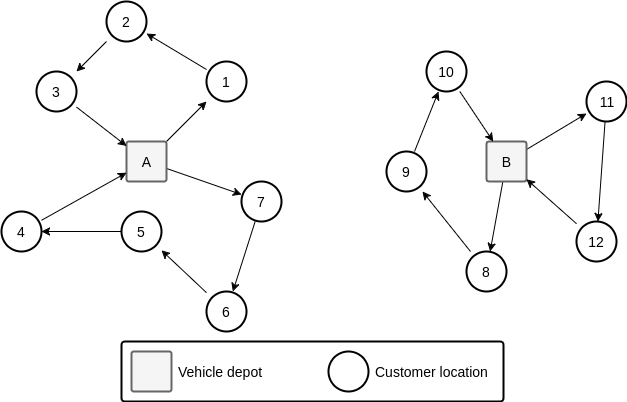
\includegraphics[width=12cm]{Resources/Images/mdvrp-illustration}
    \captionsetup{format=hang}
    \caption{Ilustrasi \textit{Multi Depot Vehicle Routing Problem}}
    \label{fig:mtsp-ilustration}
\end{figure}


Penyelesaian MDVRP bertujuan untuk mendapatkan solusi dengan total biaya terkecil. Solusi yang dihasilkan berupa sekumpulan rute dengan sejumlah konsumen yang harus dikunjungi oleh masing-masing kendaraan. Penyelesaian MDVRP harus mengikuti beberapa aturan, yaitu:

\begin{enumerate}
	\item Setiap konsumen hanya dapat dikunjungi sekali dan hanya oleh satu kendaraan. 
	\item Setiap kendaraan memulai dan mengakhiri perjalanan pada sebuah depot yang sama. 
	\item Total permintaan/\textit{demand} dari seluruh konsumen pada setiap rute tidak melebihi kapasitas dari kendaraan.
\end{enumerate}

Terdapat 2 (dua) variabel yang dapat mempengaruhi solusi atau rute yang dihasilkan, yaitu waktu tempuh antar konsumen dan lama pelayanan pada setiap konsumen. Kedua variabel ini analog dengan waktu tempuh antar wilayah kerja dan lama pencacahan dari setiap wilayah kerja pada permasalahan alokasi wilayah kerja. Lebih jauh lagi, terkait dengan terminologi yang digunakan, pencacah dapat dianalogikan sebagai kendaraan, wilayah kerja dimisalkan sebagai konsumen, dan lokasi dimana pencacah memulai perjalanan (rumah atau kantor) dapat diibaratkan sebagai depot.

Lama tempuh antar wilayah kerja dapat diestimasi dengan beberapa pendekatan, seperti melalui perkiraan, survei lokasi, atau menggunakan \textit{service} seperti Google Direction API \citep{google_google_2016}. Akan tetapi, lama pelayanan pada setiap wilayah kerja tidak dapat diketahui hingga wilayah kerja tersebut selesai dicacah. Hal ini menyebabkan rute-rute yang dihasilkan berpotensi memiliki standar deviasi dan bias yang tinggi. \autoref{fig:illustration-timeline-mdvrp} memberikan ilustrasi untuk potensi masalah ini yang dijabarkan sebagai berikut:

\begin{enumerate}
	\item Solusi yang diperoleh dengan menggunakan estimasi lama pelayanan pada setiap wilayah kerja menghasilkan rute terbaik yang relatif seimbang dari segi total waktu (\autoref{fig:illustration-timeline-mdvrp-timeservice-estimation}), 
	\item Selanjutnya, setelah semua wilayah kerja dikunjungi, ternyata lama pelayanan pada masing-masing wilayah kerja bervariasi. Lama pelayanan tersebut dipengaruhi oleh berbagai faktor seperti tingkat kesulitan medan yang dihadapi, jumlah anggota rumah tangga dalam suatu rumah tangga, dan kemampuan responden dalam menangkap maksud dari pertanyaan. Kondisi ini mengakibatkan terjadinya kesenjangan yang cukup besar terhadap total waktu pencacahan antar petugas (\autoref{fig:illustration-timeline-mdvrp-timeservice-real}).
\end{enumerate}


\begin{figure}[!]
	\centering
	\begin{subfigure}[t]{12.5cm}
		\centering
		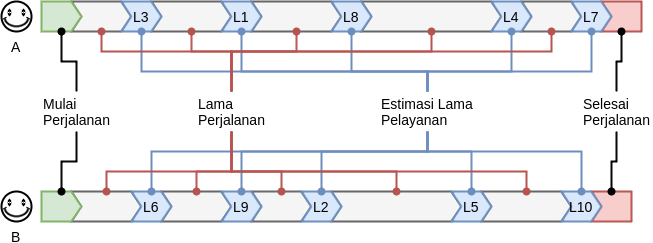
\includegraphics[width=\textwidth]{Resources/Images/illustration-timeline-mdvrp-timeservice-estimation}
		\caption{\textit{Timeline} Dengan Estimasi Waktu Pelayanan}
		\label{fig:illustration-timeline-mdvrp-timeservice-estimation}
	\end{subfigure}%
	
	\begin{subfigure}[t]{\textwidth}
		\centering
		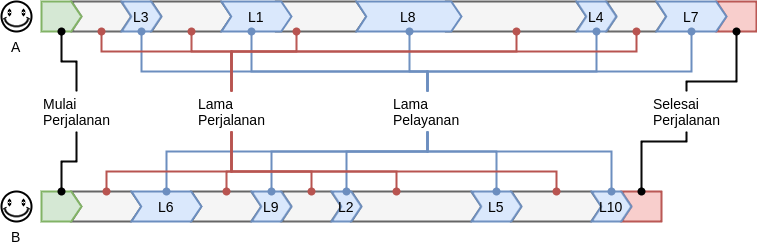
\includegraphics[width=\textwidth]{Resources/Images/illustration-timeline-mdvrp-timeservice-real}
		\caption{\textit{Timeline} Setelah Dikunjungi}
		\label{fig:illustration-timeline-mdvrp-timeservice-real}
	\end{subfigure}%
	\captionsetup{format=hang}
	\caption{\textit{Timeline} Sebelum dan Setelah Dikunjungi}
	\label{fig:illustration-timeline-mdvrp}
\end{figure}


Solusi yang ditawarkan agar rute yang dihasilkan memiliki total waktu pencacahan yang relatif setara adalah dengan menggunakan mekanisme pencarian solusi bertahap. Pada mekanisme ini setiap tahap hanya akan menghasilkan solusi/rute untuk 1 wilayah kerja yang akan dikunjungi berikutnya oleh setiap pencacah (\autoref{fig:illustration-timeline-mdvrp-gradual-solution}). 


\begin{figure}[!]
	\centering
	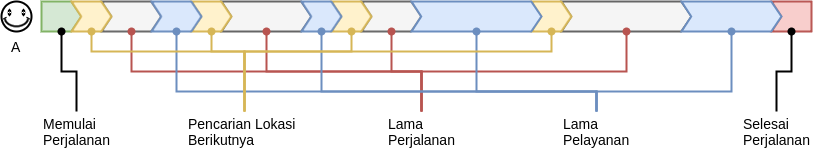
\includegraphics[width=\textwidth]{Resources/Images/illustration-timeline-mdvrp-gradual-solution}
	\captionsetup{format=hang}
	\caption{\textit{Timeline} Solusi Bertahap}
	\label{fig:illustration-timeline-mdvrp-gradual-solution}
\end{figure}


Agar `wilayah kerja berikutnya' yang dihasilkan lebih akurat, maka pencarian solusi harus dilakukan secara tersentralisasi dengan melibatkan konteks dari seluruh pencacah. Dalam sistem komputer, tidak terdapat definisi konteks yang tunggal. Sebagian besar peneliti sepakat bahwa konteks adalah sesuatu yang harus dilakukan terkait interaksi pengguna dan sistem komputer \citep{chen_survey_2000}. \citep{schilit_context-aware_1994} dan  \citep{schmidt_there_1999}, misalnya, mendefinisikan konteks sebagai pengetahuan tentang kondisi dari pengguna dan perangkat IT, termasuk lingkungan, situasi, dan lokasi. Sementara \citep{abowd_towards_1999} mendefinisikan konteks sebagai segala informasi yang dapat digunakan untuk mencirikan kondisi dari suatu entitas.


Pencarian solusi yang tersentralisasi membutuhkan mekanisme komunikasi antara \textit{client} (pencacah yang melakukan permintaan `wilayah kerja berikutnya') dan \textit{server} (pihak yang memproses permintaan dan mencari `wilayah kerja berikutnya'). Ada beragam opsi mekanisme komunikasi \textit{client-server} yang dapat digunakan, seperti \textit{Web service}, \textit{Request/Reply}, dan \textit{Publish/Subscribe} \citep{weise_solving_2009, sengoku_fast_1998, sarmenta_bayanihan_2002, muhl_large-scale_2002}. Mekanisme yang tepat diperlukan agar komunikasi antara \textit{client} dan \textit{server} dapat dilakukan dalam berbagai kondisi jaringan komunikasi.


Berdasarkan permasalahan diatas, penelitian ini dirancang untuk menciptakan sebuah sistem yang dapat digunakan dalam menentukan rekomendasi lokasi pencacahan. Peneliti mengusulkan penggunaan mekanisme pencarian solusi secara bertahap dengan mekanisme \textit{Publish/Subscribe} berdasarkan konteks dari pencacah. 


%-----------------------------------------------------------------------------%
\section{Rumusan Masalah}
%-----------------------------------------------------------------------------%
Fokus pada penelitian ini adalah bagaimana merancang sebuah sistem rekomendasi lokasi pencacahan sesuai dengan konteks dari pencacah. Adapun detail dari permasalahan yang akan dikaji adalah sebagai berikut:

\begin{itemize}
\item Bagaimana menentukan konteks dari pencacah yang cocok untuk digunakan dalam kasus rekomendasi lokasi pencacahan?
\item Bagaimana menyusun algoritma pencarian rekomendasi lokasi dengan memanfaatkan konteks dari pencacah?
\item Bagaimana menyusun mekanisme \textit{conflict resolution}, agar sistem tidak merekomendasikan lokasi yang sama pada dua atau lebih pencacah?
\item Apa mekanisme \textit{real-time} yang sesuai digunakan dalam berbagai kondisi jaringan komunikasi yang bervariasi?
\end{itemize}


%-----------------------------------------------------------------------------%
\section{Tujuan Penelitian}
%-----------------------------------------------------------------------------%
Berdasarkan rumusan masalah diatas, maka dapat ditentukan tujuan utama dari penelitian ini adalah untuk merancang sebuah sistem rekomendasi lokasi pencacahan secara \textit{real-time} berdasarkan konteks dari pencacah. 

Adapun tujuan khusus dari penelitian ini adalah:

\begin{itemize}
\item Menentukan konteks yang sesuai digunakan pada kasus rekomendasi lokasi pencacahan.
\item Menyusun algoritma rekomendasi lokasi sehingga sistem memberikan rekomendasi terbaik secara global.
\item Menyusun algoritma \textit{location conflict} sehingga tidak terjadi duplikasi rekomendasi.
\item Menganalisis dan mengimplementasikan mekanisme komunikasi yang tepat untuk digunakan pada sistem.
\end{itemize}


%-----------------------------------------------------------------------------%
\section{Batasan Masalah}
%-----------------------------------------------------------------------------%
Masalah dalam penelitian ini memiliki batasan sebagai berikut:

\begin{itemize}
\item Lokasi pencacahan yang menjadi rujukan adalah Blok Sensus (BS) yang dikeluarkan oleh Badan Pusat Statistik (BPS).
\item Penelitian tidak berfokus pada algoritma MDVRP, sehingga pengujian hanya dilakukan dengan menggunakan salah satu algoritma MDVRP.
\end{itemize}


%-----------------------------------------------------------------------------%
\section{Manfaat dan Kontribusi}
%-----------------------------------------------------------------------------%
Hasil penelitian ini diharapkan dapat memberikan kontribusi secara khusus kepada BPS, berupa kemudahan bagi \textit{subject matter} dalam melakukan alokasi petugas pencacahan. Ketepatan alokasi petugas memiliki implikasi pada seimbangnya beban setiap pencacah serta meratanya waktu penyelesaian pencacahan.

Sistem yang dihasilkan di dalam penelitian ini tidak hanya dapat digunakan secara spesifik untuk kasus pengumpulan data, tetapi juga dapat digunakan pada kasus lain terkait dengan \textit{Vehicle Routing Problem}. Ditinjau dari prospek pemanfaatannya yang luas, penelitian ini diharapkan dapat memberikan sumbangsih terhadap kemajuan bidang akademis. 

%-----------------------------------------------------------------------------%
\section{Sistematika Penulisan}
%-----------------------------------------------------------------------------%
Sistematika penulisan tesis ini terdiri atas enam bab dengan perincian sebagai berikut:


BAB I PENDAHULUAN. Pada bab ini dijelaskan fenomena dan masalah yang diangkat dalam penelitian ini. Selain itu, dipaparkan pula mengenai rumusan masalah, tujuan penelitian, dan kontribusi penelitian.


BAB II STUDI LITERATUR. Bab ini menjelaskan landasan teori yang digunakan dalam penelitian, teknologi pendukung, serta penelitian terkait dengan penelitian yang dilakukan.


BAB III METODOLOGI PENELITIAN. Pada bagian ini dijelaskan metode penelitian yaitu alur dan langkah-langkah dalam melakukan penelitian.


BAB IV ANALISIS DAN PERANCANGAN. Bab ini memaparkan analisis terhadap permasalahan yang dihadapi, serta kriteria yang dibutuhkan pada algoritma yang dirancang. Dari analisis permasalahan, diuraikan pendekatan yang dibuat yang merupakan solusi atas permasalahan yang dikemukakan.


BAB V IMPLEMENTASI DAN PENGUJIAN. Proses dan hasil implementasi rancangan dijelaskan dalam bab ini. Proses pengujian diuraikan mulai dari skenario pengujian hingga hasil pengujian.


BAB VI KESIMPULAN DAN SARAN. Bab ini memaparkan kesimpulan yang diperoleh dari penelitian ini, serta saran untuk pihak terkait dan penelitian selanjutnya yang berkaitan dengan topik penelitian ini
